\begin{enunciado}
 Se extraen 3 cartas de una baraja ordinaria, con reemplazo,
 y se registra el n\'umero $Y$ de espadas.
 Despu\'es de repetir el experimento $64$ veces, se registran
 los siguientes resultados:
 \begin{center}
  \begin{tabular}{c|cccc}
   $y$ & $0$ & $1$ & $2$ & $3$ \\
   \hline
   $f$ & $21$ & $31$ & $12$ & $0$
  \end{tabular}
 \end{center}
 Con un nivel de significancia de $0.01$, pruebe la hip\'otesis
 de que los datos registrados se pueden ajustar
 mediante la distribuci\'on binomial $b(y;3,1/4)$, $y=0,1,2,3$.
\end{enunciado}

\begin{solucion}
 \begin{datos}
  $\phantom{0}$
  \begin{itemize}
   \item Tama\~no de la muestra: $n=64$.
   \item Frecuencias observadas: $O = \{o_0=21, o_1=31, o_2=12, o_3=0 \}$.
   \item Probabilidades esperadas: $p_i = 
   \binom{3}{i}\left(\frac{1}{4}\right)^i\left(\frac{3}{4}\right)^{3-i}$,
   para cada $i \in \mathbb{Z}\cap[0,3]$.
   Entonces $p_0 = \frac{3^3}{4^3} = \frac{27}{64}$,
   $p_1 = \frac{3\cdot 3^2}{4^3} = \frac{27}{64}$,
   $p_2 = \frac{3 \cdot 3}{4^3} = \frac{9}{64}$ y 
   $p_3 = \frac{1}{4^3} = \frac{1}{64}$.
   \item Frecuencias esperadas: $E = \left\{
   \left.e_i=n\cdot p_i\,\right|\,\forall i\in\mathbb{Z}\cap[0,3] \right\}
   = \{e_0 = 27, e_1 = 27, e_2 = 9, e_3 = 1 \}$.
  \end{itemize}
  Dado que las pruebas de bondad por m\'etodo de $\chi^2$ no son confiables
  cuando la frecuencia esperada de una celda es menor a $5$,
  se agrupar\'an los datos, como sigue:
  \begin{itemize}
   \item Probabilidades esperadas:
   $\{ p_0 = \frac{27}{64}, p_1 = \frac{27}{64}, p_2 = \frac{10}{64} \}$.
   \item Frecuencias esperadas: $E=\{e_0 = 27, e_1 = 27, e_2 = 10\}$.
   \item Frecuencias observadas: $O=\{o_0 = 21, o_1 = 31, o_2 = 12\}$.
   \item Celdas totales del experimento: $k=3$.
   \item grados de libertad de la prueba $\chi^2$: $v= k-1 = 2$.
  \end{itemize}
 \end{datos}
 
 \begin{hipotesis}
  Prueba de bondad de ajuste para probar $H_0:$
  que la variable aleatoria $Y$ del n\'umero de espadas
  al extraer $3$ cartas con reemplazo del mazo del enunciado
  sigue una distribuci\'on binomial con par\'ametro $p=\frac{1}{4}$,
  contra la alternativa $H_1$ de que no es as\'{\i}.
 \end{hipotesis}

 \begin{significancia}
  $\alpha = 0.01$.
 \end{significancia}

 \begin{region}
  De la tabla A.5 se tiene el valor cr\'{\i}tico
  $\chi^2_{\alpha,v} = \chi^2_{0.01,2} \approx 9.21$,
  por lo que la regi\'on de rechazo est\'a dado
  para $\chi^2 > 9.21$, donde
  $\chi^2 = \sum_{i=0}^{k-1} \frac{\left( o_i - e_i \right)^2}{e_i}$.
 \end{region}

 \begin{estadistico}
  \begin{eqnarray*}
   \chi^2 & = & \sum_{i=0}^{k-1} \frac{\left( o_i - e_i \right)^2}{e_i}
   = \frac{(21-27)^2}{27} + \frac{(31-27)^2}{27} + \frac{(12-10)^2}{10}
   = \frac{6^2(10) + 4^2(10) + 2^2(27)}{270} = \frac{628}{270} \\
   & = & \frac{314}{135} = 2.3\overline{259}
  \end{eqnarray*}
 \end{estadistico}

 \begin{decision}
  No se rechaza $H_0$.
 \end{decision}

 \begin{conclusion}
  Se confirma que el n\'umero de espadas obtenidas al extraer $3$ cartas
  con reemplazo del mazo del enunciado sigue una distribuci\'on
  que no es significativamente distinto al de una binomial
  con par\'ametro $p = \frac{1}{4}$.
 \end{conclusion}

 Finalmente, usando el archivo anexo
 \texttt{P15\_Prueba\_de\_bondad\_chi2\_01.r},
 que a su vez requiere los datos del archivo
 \texttt{DB19\_Problema\_083.csv}, con los siguientes cambios:
 \begin{verbatim}
> datos<-read.csv("DB19_Problema_083.csv",sep=";",encoding="UTF-8")
> varInteres<-"Frecuencia"
> varCelda<-"Conteo.cantidad"
> distribucion<-2
> parametro_nombre<-c("p")
> parametro_valor<-c(1/4)
> combinar<-TRUE
> grafica<-TRUE
> tituloEjeX<-"Primera aparición de espadas al sacar 3 cartas con reemplazo"
> alfa<-0.01
 \end{verbatim}
 \vspace{-0.5cm}
 el programa de R lanza el siguiente resultado:
 \begin{verbatim}
         Variable Distribución de ajuste    p Estadístico Chisq2
1 Conteo.cantidad               Binomial 0.25           2.325926
  Grados de libertad   Valor-p alpha Región de Rechazo
1                  2 0.3125587  0.01       > 9.2103404
                          Resultado
1 No se rechaza el ajuste de bondad
 \end{verbatim}
 \vspace{-0.5cm}
 que incluye la siguiente figura:
 \begin{center}
  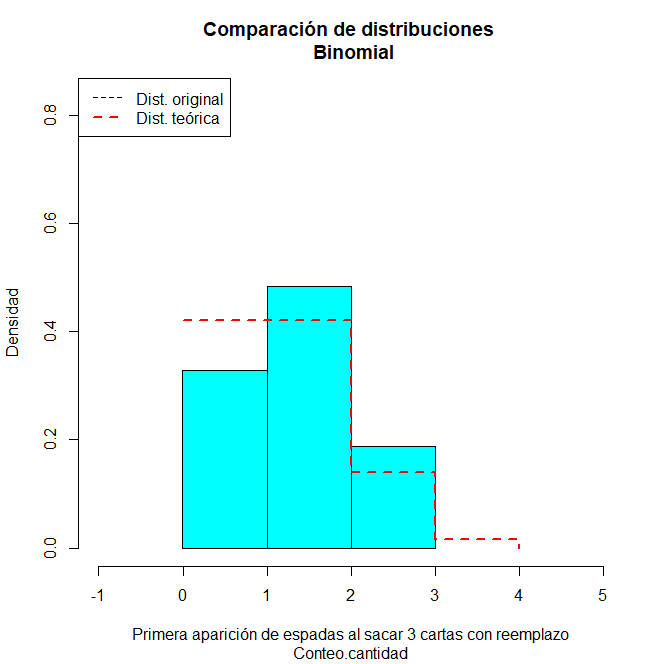
\includegraphics[scale=0.35]{Problema_83.png}
 \end{center}
 El cual coincide con los datos obtenidos,
 que es a lo que se quer\'{\i}a llegar.${}_{\blacksquare}$
\end{solucion}
